\section{Methods}

This section will provide introductory information about how to set up the two different experiments, and how to collect and process the data from the instruments used. Procedures for working in situ are presented as well as some preliminary conditions for doing measurements, namely that the sea ice is stable, and naturally grown.

\subsection{Instruments}
A short list of equipment needed for doing salinity evolution measurements

\addtokomafont{labelinglabel}{\sffamily}
\begin{labeling}{Lists}
  \item [Ice saw] 2 meter long foldable saw that allows its user to cut the ice with ease
  \item [Ice drill] motorised drill used to create the starting points for the ice saw when constructing larger ice holes
  \item [Wire harp] measurement device with two horizontally spaced titanium wires and a temperature sensor placed vertically at eight different depths
  \item [Stand] a wooden construction created on site to hold the instrument in place during the experiment
  %\item [Ice core kit] containing a manual ice core drill for drilling and extracting ice cores, a plastic tube cut in half across its length for holding the ice core in place when performing ice core measurements. Kit also contains a measuring stick, temperature sensor, drill, saw, and plastic bags for storage. 
\end{labeling}

%%%%%% REWRITE Z0 FUNCTION PART
\subsection{Procedure}
The goal of the experiment is to collect data on the salinity evolution in growing sea ice, and in snow above the ice, by using a relatively new instrument called a wire harp. The instrument has been used for similar purposes in both 2016 and 2017 in context with the AGF-211 fieldwork. To measure the salinity evolution in growing sea ice the harp was placed in a hole with dimensions $ 130 \text{cm} \pm 5\text{cm} \times 140 \text{cm} \pm 5\text{cm}$. Then, every part of the instrument from the wooden stand to the harp itself was secured to the ice with rope and ice screws, in case of any accidents. Then plan for the experiment was to let the sea ice refreeze the first night, and then begin a snow experiment on top of the newly grown sea ice the following day. Due to the snow experiment the placement of the harp in the water was therefore of great importance. The harp deliberately not submerged completely in water. Instead, two wire pairs were placed above the water, and one wire pair just below the water surface. Regarding the snow experiment, the plan was to cover the harp with an even amount of 15 cm of snow to create a freeboard negative enough, so that there would be some flooding. The thin sea ice however, was not strong enough to support such a huge load, and this led to immense flooding through almost all of the snow. Because wet snow also means that the there will be an even greater load on ice, around half of the snow was removed shortly after. The new snow height after this was $7 \text{cm} \pm 1\text{cm}$ (of wet snow). After that the experiment was left untouched for the remainder of the fieldwork. The instrument set-up can be seen in detail in \autoref{icehole1}.

The other harp was placed directly on the ice surface with the bottom wires touching the ice. Around the harp there was built a wall of ice blocks to ensure negative freeboard in the test area. Then, snow  was distributed evenly around and above the harp, to a height of approximately 30 cm. After that the project was left untouched for the remainder of the fieldwork.

The snow used in both experiments was not snow gathered from the sea ice (which is salty), instead it was gathered from the base of a tiny mountain nearby. After both experiments was finished and packed up, a piece of the newly grown sea ice was sawed out for comparison, and a snow analysis of the snow experiment was done to obtain grain sizes. Other than that, and in order to ensure that the harp was working and recording data at all times, the battery capacity was checked once a day, along with downloading data from the data logger at the same time.

\begin{figure}[h!]
\centering
	\begin{subfigure}{0.4\linewidth}
		\centering
		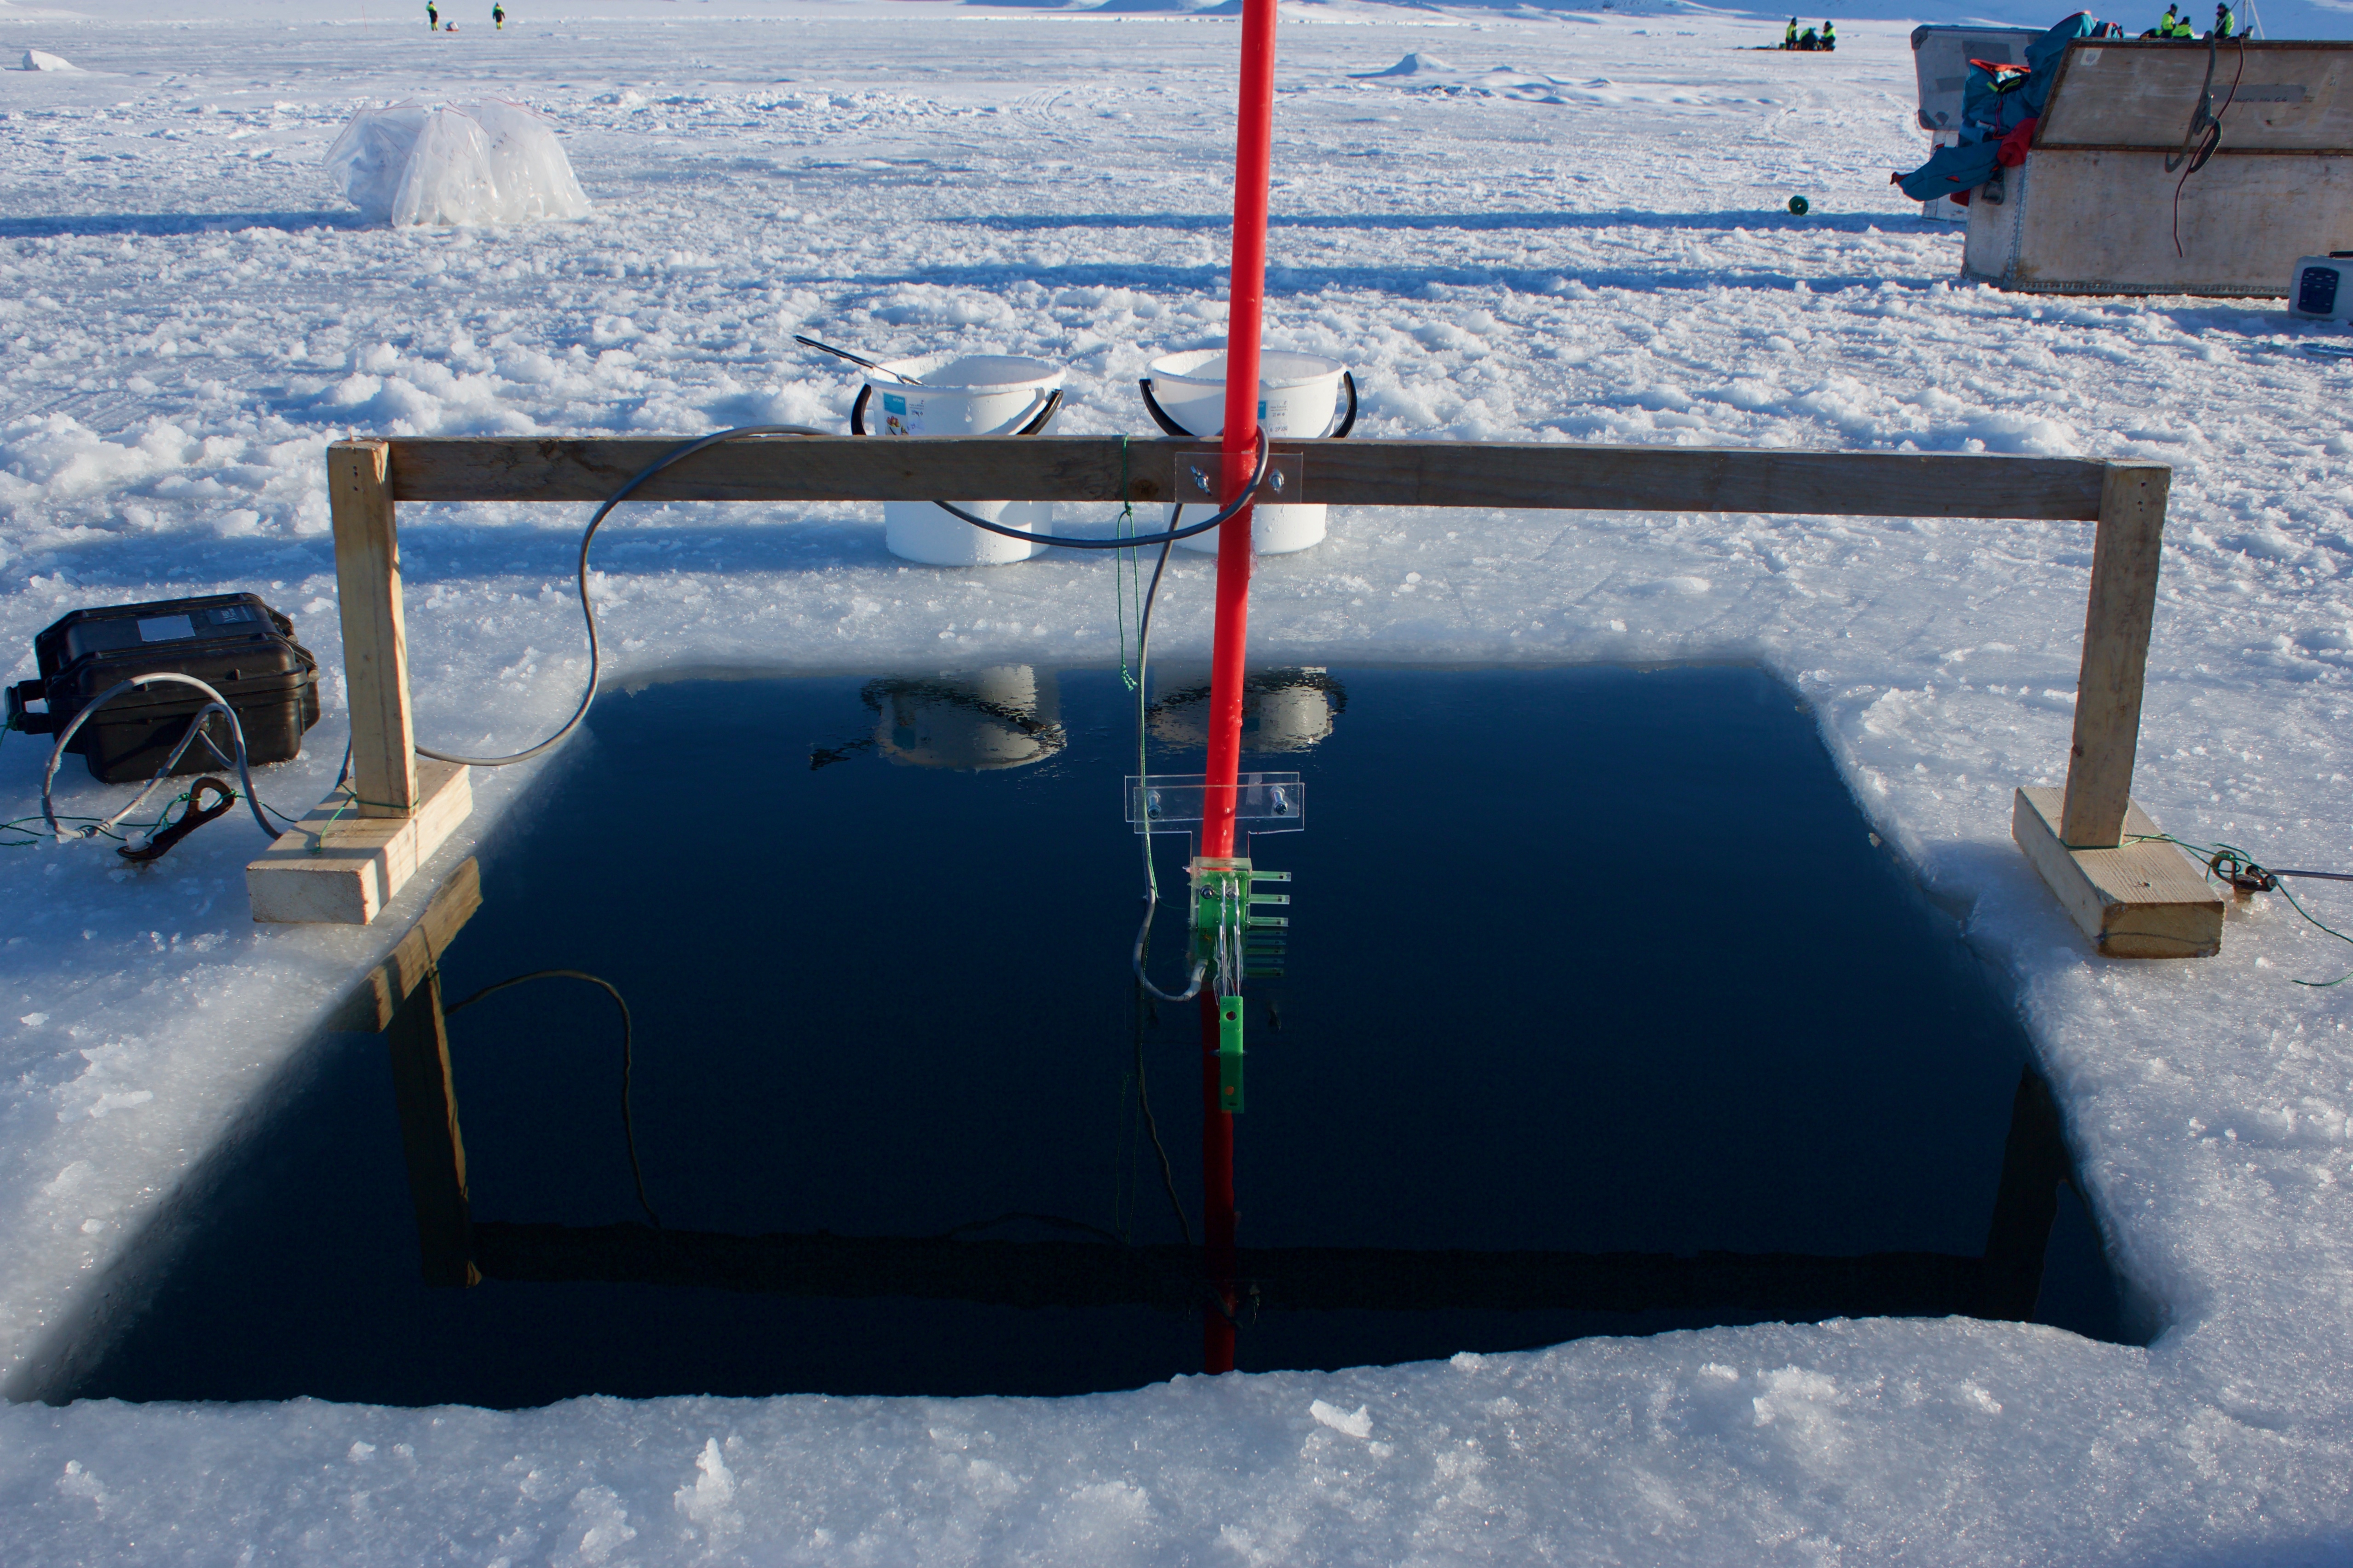
\includegraphics[width=0.9\linewidth]{MG_6752}
		%\caption{(a)}
	\end{subfigure}\quad
	\begin{subfigure}{0.4\linewidth}
		\centering
		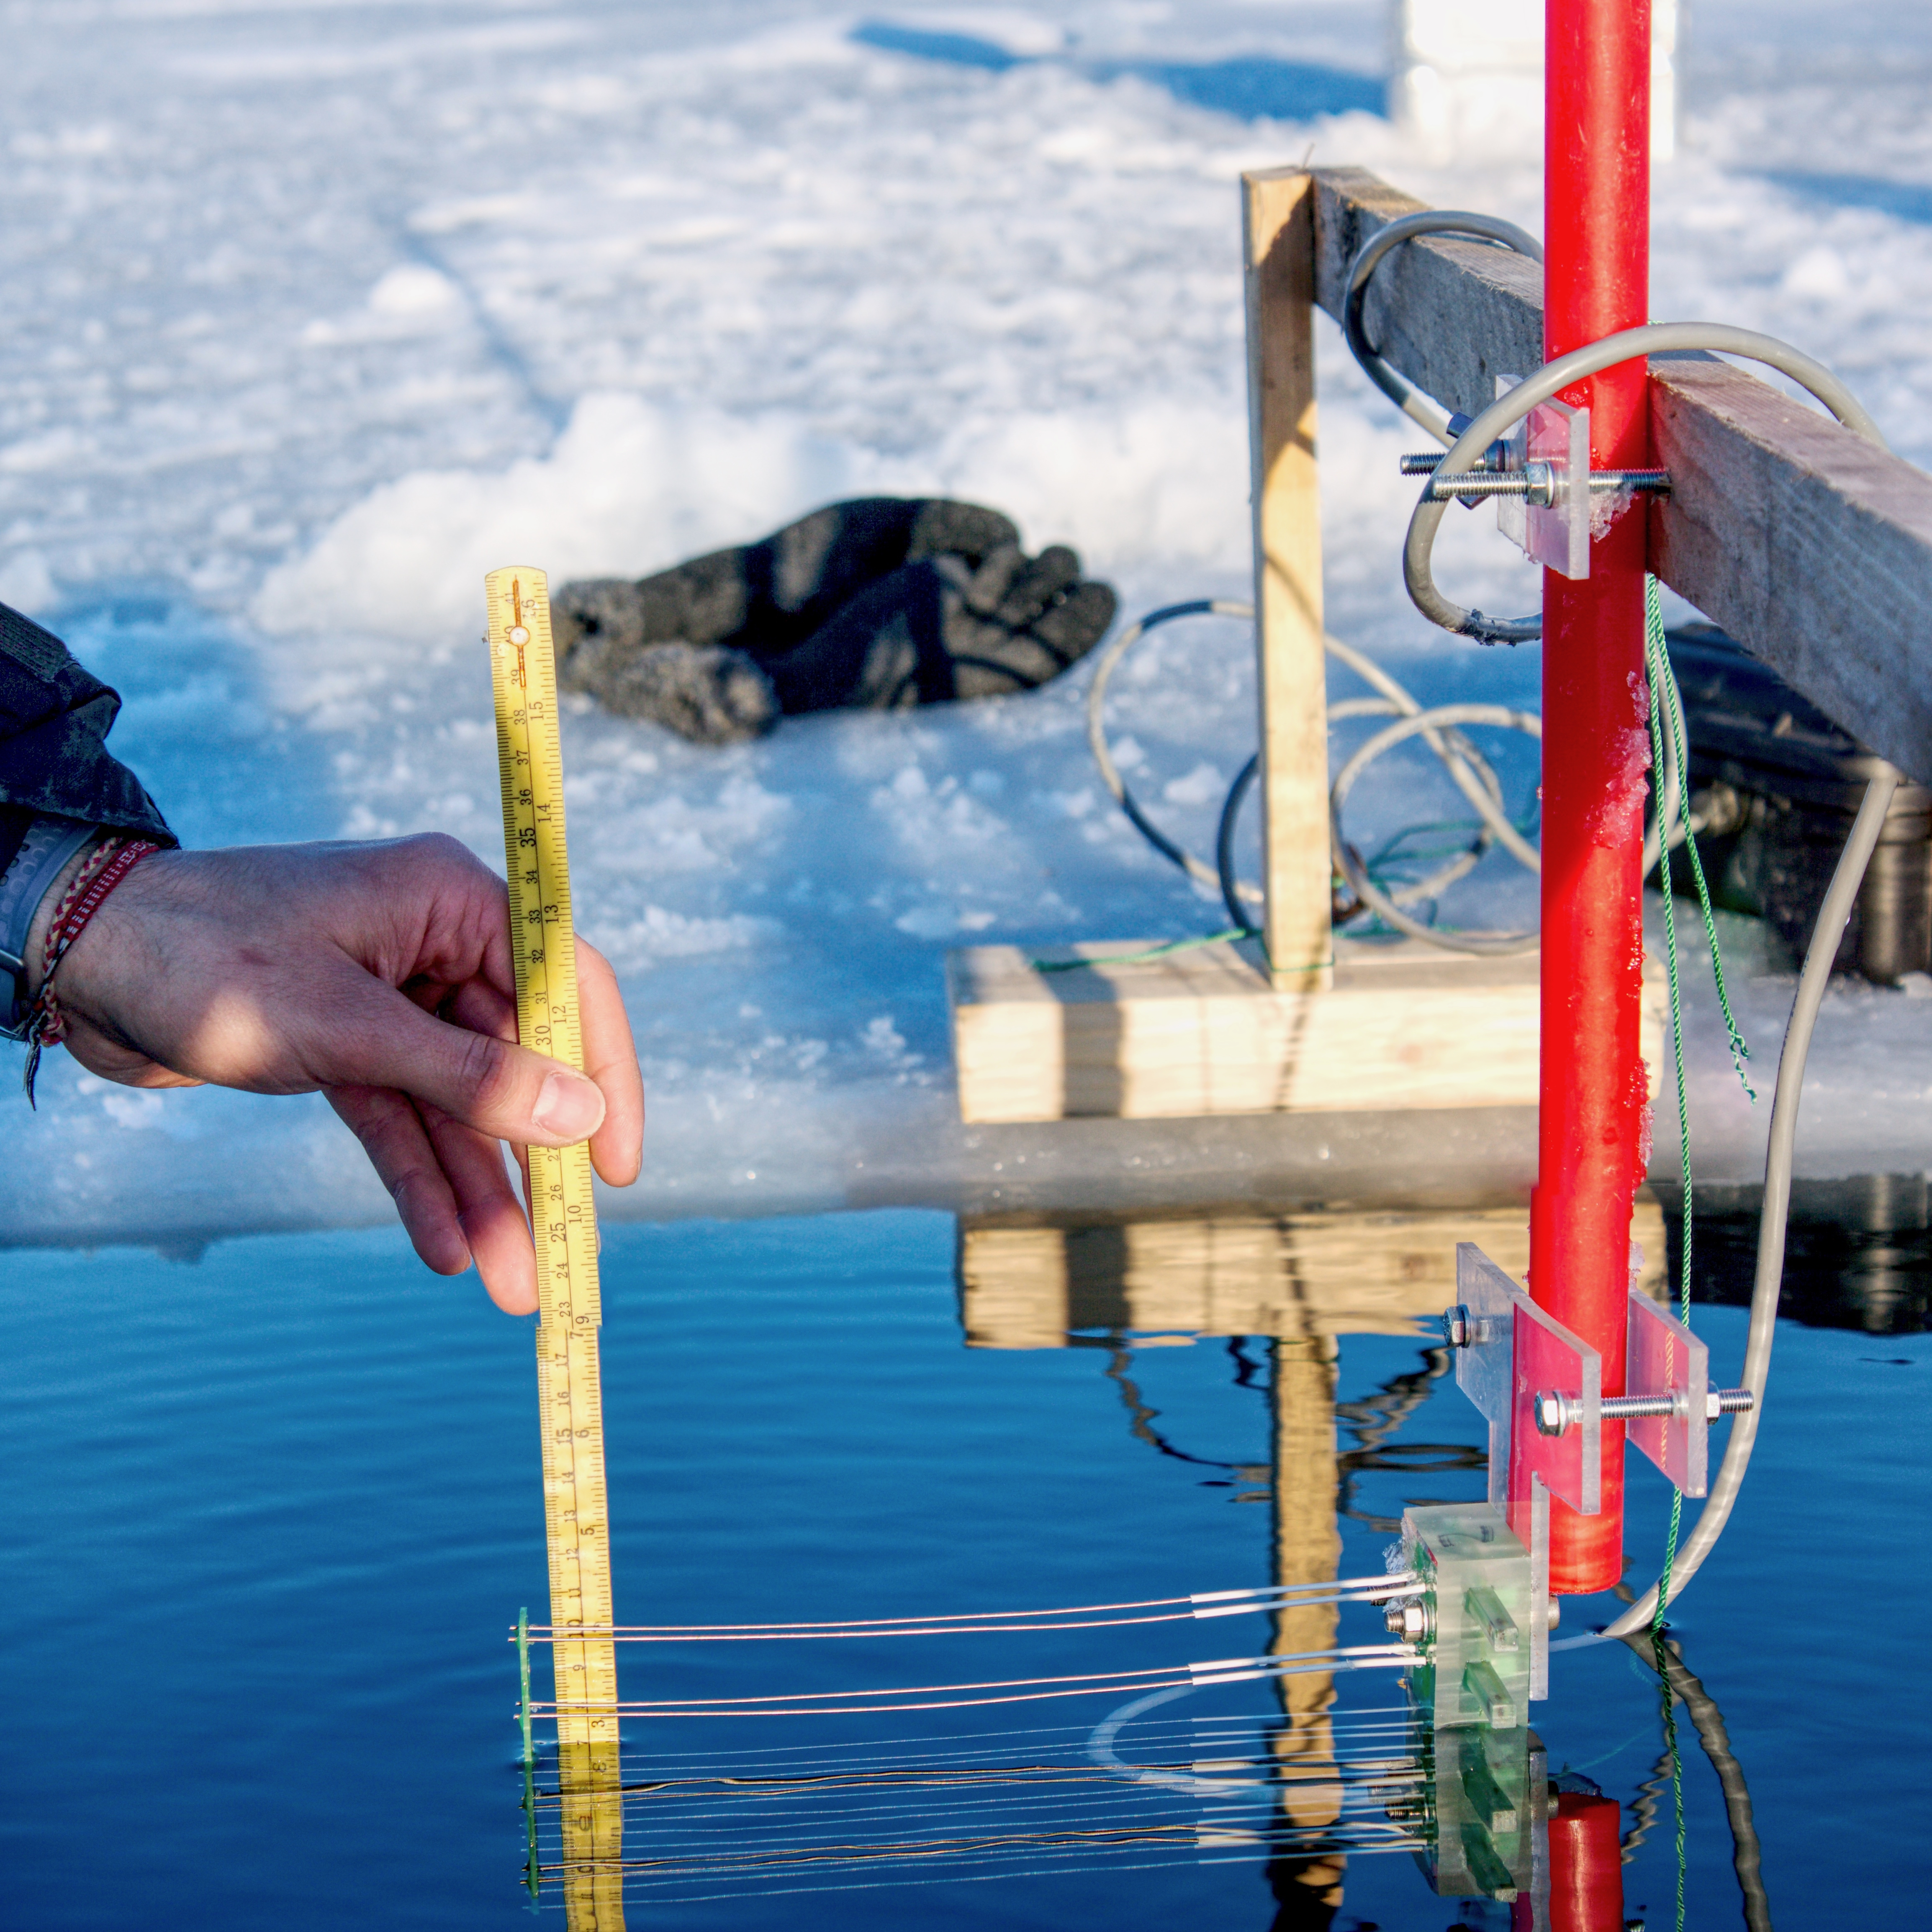
\includegraphics[width=0.7\linewidth]{Harp_in_water}
		%\caption{(b)}
	\end{subfigure}
\caption{The whole instrument set-up can be seen in the image to the left, and the harps exact placement in water can be seen in the image to the right.}
\label{icehole1}
\end{figure}

\begin{figure}[h!]
\centering
	\begin{subfigure}{0.4\linewidth}
		\centering
		\includegraphics[width=0.9\linewidth]{aleks_1}
		%\caption{(a)}
	\end{subfigure}\quad
	\begin{subfigure}{0.4\linewidth}
		\centering
		\includegraphics[width=0.9\linewidth]{aleks_2}
		%\caption{(b)}
	\end{subfigure}
\caption{The snow set-up can be seen in the image to the left, the picture to the right shows how the snow was applied.}
\label{snowsite}
\end{figure}


\subsubsection{The wire harp}
The wire harp is an instrument that measure the impedance($\text{Z}(\text{t})$) and temperature ($\text{T}(\text{t})$) at different height over time (\text{t}). The type of harp used in the experiment was first introduced by \textcite{Notz}. As the wire harp have for the past years still been in development, they all look a bit different. This years harps had an improvement in overall build quality and reliability, compared with earlier models used in \textcite{2017icegrowth}, \textcite{2016icegrowth}, and \textcite{2016snow}.

The harp used this year had 8 pairs of wires spaced out with a vertical distance of 2 cm between each wire pair. The harp measures the impedance between the two wires in a pair with a frequency of two and sixteen kHz respectively. As found by \textcite{Fuchs},the most reliable setting for this type of experiment is the two kHz setting. The Harp used this year mounted on its wooden stand can be seen in \autoref{Harp}.

\begin{figure}[h!]
\centering
	\begin{subfigure}{0.4\linewidth}
		\centering
		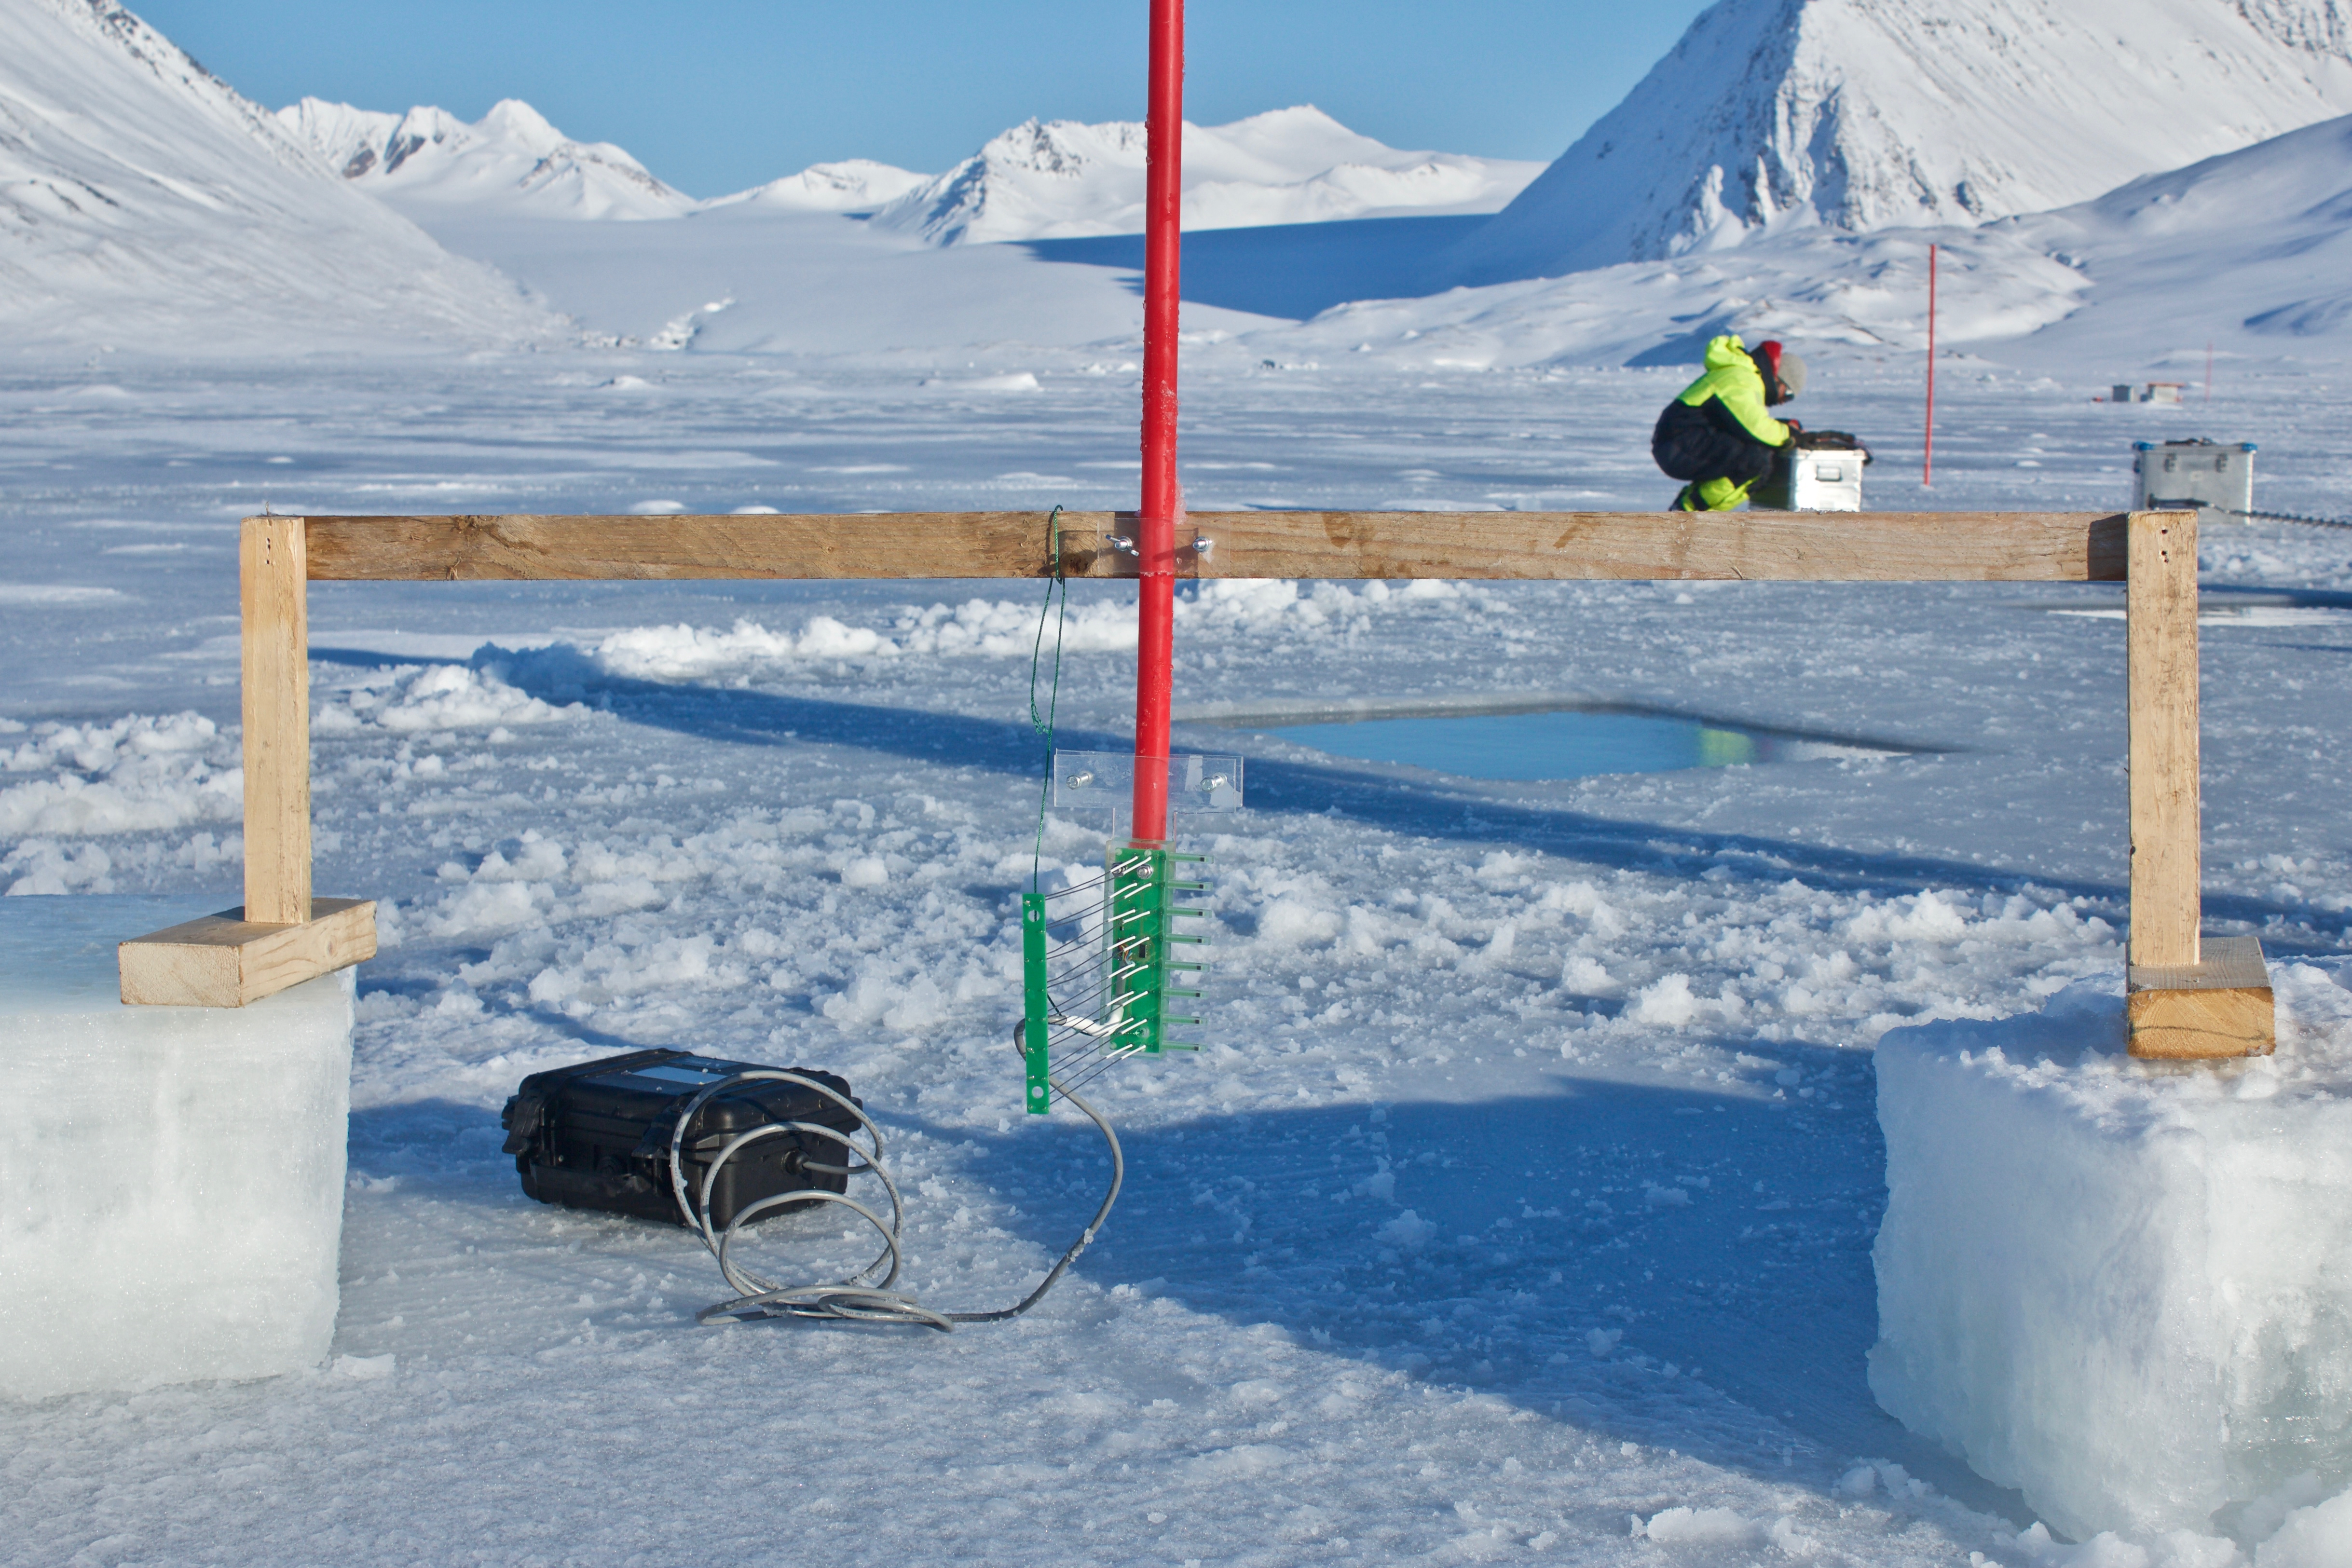
\includegraphics[width=0.7\linewidth]{_MG_6729}
		%\caption{(a)}
	\end{subfigure}\quad
	\begin{subfigure}{0.4\linewidth}
		\centering
		\includegraphics[width=0.9\linewidth]{Harp_about}
		%\caption{(b)}
	\end{subfigure}
\caption{Image to the left displaying one of the harps used in the experiment. The harps data logger is protected inside the black box that can be seen in the background. Image to the right is a sketch of the harp measurement principle \textcite{Fuchs}. Here the harp is mounted close to the water surface where the sea ice starts to form around the harp. Light blue is the Solid ice ($\phi_{\text{s,v}}$). Dark blue is the scattered liquid brine channels($\phi_{\text{l,v}}$). The white modules that can be seen on the left display the temperature sensors. }
\label{Harp}
\end{figure}

%\subsubsection{Ice core measurements}
%ICE CORE discussion form Fuchs

\subsection{Techniques}
The following sections contain topics on the post-field data gathering and analysis.

\subsubsection{Data and Plots}
Python (v2.7), as well as MATLAB (R2017b) was used for data processing and producing figures. In Python for interpreting the data the Pandas, Datetime and the Numpy packages was used, and for plotting the Matplotlib package was used. Both the code used, and data gathered are available on the UNIS server.\\
\\
Upon first looking in to the data, there where some significant spikes in the data whenever the harp was turned on after reading out the data, this was mainly a problem on the snow harp, and after email correspondence with the technician who built the harp, it was discovered that it cannot measure reliably over $17000 \Omega$. As the top wire of the harp used in the snow experiment never gave any data under this, it was removed from that dataset. Furthermore, data recorded from a test done before the cruise, as well as all data recorded after the experiments had been concluded have also been removed. This includes data logged from one final test on the ship, that were done as a precaution and because of the mentioned spikes, as we did not know about the said limit at this time.\\
\\
To avoid strange interpolation in some of the plots, data was removed where it was needed to do so to avoid this. This was mainly the case for the sea ice harp, where two of the wire pars was first in air, and then covered in snow. Interpolation caused there to be values where the values were supposed to be zero for when the wires were in the air.\\ 
\\
Another important note to make regarding the plotting, is that when plotting the data as a function of the depth, the sensor that was placed just below the surface was assumed to be at the surface, and every other sensor shifted in relation to that one. 

\subsubsection{Background and Theory}
%Data interpretation\\
From the impedance and temperature measured it is possible to calculate salinity and solid/liquid fractions. The formulas used for this originally appeared in \textcite{Notz}, formulas that later have been updated for the modern harps in \textcite{Fuchs}. The equation used can be found there. The only notable difference is that for both harps the lowest values of impedance for each wire pair was chosen as
$Z_0$, which is the impedance in liquid water before ice starts to freeze. This deviates from the method proposed by \textcite{Fuchs}. The reason for this is that finding the value for $Z_0$ in case of the snow experiment there is never no snow/ice and therefore the lowest value is the most correct one. While it for the sea ice experiment proved difficulties implementing into a the MATLAB scripts already written.\\ 
\\
Regarding the snow experiment it is known that Darcy's law describes the flow of a fluid through a porous medium, and can be used to describe brine percolation through snow. From that a one dimensional version of the law can be written as:
\begin{equation}
  q = -\frac{\kappa}{\mu}\Delta p
\end{equation}
here q is the flux given as [m/s], $\kappa$ is the permeability of the material, $\mu$ is the viscosity of the fluid, and $\Delta p$ is the difference in pressure as a function of height.\\
\\
The Young-Laplace equation describes the pressure difference known as capillary pressure, due to the wetting between two fluids and can be described as:
\begin{equation}
  \Delta p = \gamma \left( \frac{1}{\text{R}_1} + \frac{1}{\text{R}_2} \right) = \frac{2\gamma cos\theta}{\text{R}_\text{c}}
\end{equation}
Where $\Delta p$ is the pressure difference, $\gamma$ is the surface tension, $R_1, R_2$ are the principle radii of curvature, $\theta$ is the wetting angle and $\text{R}_\text{c}$ is the radius of a capillary tube. When there is a horizontal difference between the points $\Delta p$ needs to me divided by $\rho g$ where $\rho$ is the density and $g$ is the gravitational acceleration.

%you describe the theory or method behind your estimations of specific values that you present in the results\\
%– such as salinity calculations\\
%– other things\\
%Definitions or a list of abbreviations can be given in the end (i.e. before the Appendix)\\
\begin{table}[h!]
\centering
\begin{tabular}{c|c}
Variable      & Standard Deviation      \\ \hline
Temperature   & $\pm$ 0.15 \\
Bulk Salinity & $\pm$ 1.76
\end{tabular}
\caption{Table showing uncertainties in measurements.}
\label{uncertainties}
\end{table}

\subsection{Uncertainty}
The Measurement accuracies for the harp is listed in Table \autoref{uncertainties}, and is only is for the two kHz frequency, and was originally presented in \textcite{Fuchs}. For an in-depth look at the uncertainties, and how these were calculated the reader is refereed to that master thesis. 

As mentioned the value we used for $Z_0$ was not the same as the method proposed to calculate it in \textcite{Fuchs}. The impact of this deviation hard to quantify. Through the examination of the the raw data this would only affect one of the wires, and only in the case of the sea ice experiment. In addition rapid ice growth in the beginning also reduces the uncertainty related to the $Z_0$ as the wire that was affected was the second one from the surface. This is all just assumptions and speculations, and it could turn out that the impact is greater predicted above. It is nevertheless important to be aware of the potential error.\\
\\
Another factor that greatly impacts the experiment is the weather and the environment. As the very nature of the experiment is on the on the see ice outside, one cannot hope to get a stable environment with total control of all the factors that affect sea ice growth. With the help of all the data collected with other experiments, there is a great possibility to explain some of these impacts. Nonetheless, to know for sure the experiments must be carried out.\\
\\
Furthermore, another uncertainty is the risk of animals, helicopters and people disturbing the experiment in a variety of ways from physical destruction to flooding. The thicker the ice, the more resilient it is to such disturbances. Since the a great deal of the experiment is focused around thin ice, this means that precautions must be made so that such disturbances will not disturb and or destroy the experiment.
What's more, is that the impact of such disturbances is hard to quantify, as one can't exactly be inside the sea ice and witness these changes happening.\\
\\
At last, another huge uncertainty, which also has to do with the fact that the experiment is carried out outdoors, is the snow experiments. When those experiments were carried out, no thoughts were put into finding out how much negative freeboard would be needed to get sufficient sea water flooding in the snow, or how much snow the newly grown sea ice actually could hold. The impact of this \enquote{ignorance} is hard to tell. At least the results got more interesting, but not necessary more useful for future comparisons. 

%Uncertanty for all the mesaurements from length measurements, to the harps speciffic mesaurements, weight uncertanty
%and general uncertany about the experiment. Things that can affect, and that is hard to prevent

%past and passive, include references
%------
%'Exeeds Standard' criteria for Report Grading:
% The Methods includes detailed graphical and textual descriptions of all instruments and procedures, such that a competent outsider could reproduce every aspect of the study.
%------
